\sectioncounter{7}
  \section{指数式与指数函数}

  \subsection{知识梳理}
  
  指数式的三个基本运算律如下:
  \[a^m\cdot a^n= a^{m+n},\quad (a^m)^n= a^{mn},\quad (ab)^n= a^n b^n,\]
  其中 $m$, $n\in\mathbb{R}$, $a$, $b>0$. 由第一式可知 
  $\frac{a^m}{a^n}= a^{m-n}$, 故定义 
  \[a^0= a^{1-1}=\frac{a}a= 1,\quad 
    a^{-n}= a^{0-n}=\frac{a^0}{a^n}= \frac1{a^n},\]
  表明正数的零次方一定是 $1$, 而指数中负号的意思是 ``取倒数''.
  注意, 零的零次方没有定义.
  再由 $(\sqrt[n]{a})^n= a$ 和第三个基本运算律, 可定义 
  \[a^{\frac1n}= \sqrt[n]{a},\]
  即指数中的分母意味\myemph{开方运算}.
  
  形如 $y=a^x$ 的函数称为\myindex{指数函数} (exponential function), 
  \mymarginpar{任意两个指数函数的图象有且仅有一个公共点 $(0,1)$. 由 $y=a^x$ 的图象估计底数 $a$ 的值时, 只需考虑 $x=1$ 时的函数值.}
  其中 $a>0$ 且 $a\neq1$. 分别考虑指数函数 $y= 2^x$ (如图~\ref{fig-190126-2340}) 和 $y=\Big(\frac12\Big)^x$ (如图~\ref{fig-190126-2345}) 的图像可以知道, 指数函数 $y=a^x$ 恒过点~$(0,1)$, 并以直线 $y=0$ 即 $x$~轴为渐近线, 且当 $0<a<1$ 时单调递减, 而当 $a>1$ 时单调递增. 指数函数没有奇偶性, 而 $y=a^x$ 与 $y=\Big(\frac1a\Big)^x$ 的图象关于 $y$ 轴对称 (后者可以写为 $y=a^{-x}$).
  \mymarginpar{对下图中的四个指数函数图象, 借助 $x=1$ 可知 $0<d<c<1<b<a$.
    \begin{center}
    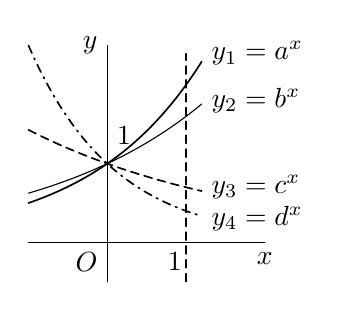
\begin{tikzpicture}[line cap=round,line join=round,scale=1]
      \draw[\myaxisarrow] (-1,0) -- (2,0) node[below] {$x$};
      \draw[\myaxisarrow] (0,-0.5) -- (0,2.5) node[left] {$y$};
      \draw[line width=0.6pt,smooth,samples=100] 
        plot[domain=-1:1.2](\x,{2^(\x)});
      \draw[line width=0.4pt,smooth,samples=100] 
        plot[domain=-1:1.2](\x,{1.6^(\x)});
      \draw[line width=0.6pt,smooth,samples=100,densely dashed] 
        plot[domain=-1:1.2](\x,{0.7^(\x)});
      \draw[line width=0.6pt,smooth,samples=100,dash dot] 
        plot[domain=-1:1.2](\x,{0.4^(\x)});
      \draw[densely dashed] (1,-0.5)--(1,2.4);
      \draw (0,0) node[anchor=north east] {$O$}
        (1,0) node[below,xshift=-4pt] {$1$} 
        (0,1) node[right,yshift=10pt] {$1$}
        (1.2,2.4) node[right] {$y_1=a^x$} (1.2,1.8) node[right] {$y_2=b^x$}
        (1.2,0.7) node[right] {$y_3=c^x$} (1.2,0.3) node[right] {$y_4=d^x$};
    \end{tikzpicture}\end{center}}
    
  \begin{figure}[htb]
  \small\centering
  \begin{minipage}[b]{0.4\linewidth}
  \centering
  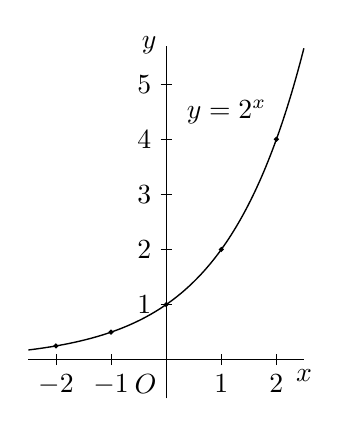
\begin{tikzpicture}[scale=0.7]
    \draw[\myaxisarrow] (-2.5,0)--(2.5,0) node[below] {$x$};
    \draw[\myaxisarrow] (0,-0.7)--(0,5.7) node[left] {$y$};
    \draw (0.2,4.5) node[right] {$y=2^x$};
    \draw[line width=0.5pt,smooth,samples=100,domain=-2.5:2.5] plot(\x,{2^(\x)});
    \foreach \x in {-2,-1,1,2}
      {\draw[line width=0.2pt] (\x,-0.1) node[below] {$\x$} --(\x,0.1);}
    \foreach \y in {1,2,...,5}
      {\draw[line width=0.2pt] (-0.1,\y) node[left] {$\y$}--(0.1,\y);}
    \draw (0,-0.1) node[anchor=north east] {$O$};
    \draw [fill=black] (0,1) circle (1pt) (-1,0.5) circle (1pt)
      (-2,0.25) circle (1pt) (1,2) circle (1pt)
      (2,4) circle (1pt);
  \end{tikzpicture}
  \caption{}\label{fig-190126-2340}
  \end{minipage}
  \hskip 1cm%
  \begin{minipage}[b]{0.4\linewidth}
  \centering
  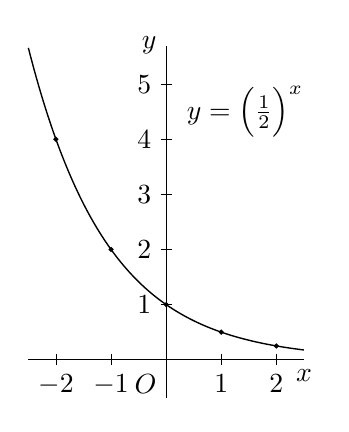
\begin{tikzpicture}[scale=0.7]
    \draw[\myaxisarrow] (-2.5,0)--(2.5,0) node[below] {$x$};
    \draw[\myaxisarrow] (0,-0.7)--(0,5.7) node[left] {$y$};
    \draw (0.2,4.5) node[right] {$y=\Big(\frac12\Big)^x$};
    \draw[line width=0.5pt,smooth,samples=100,domain=-2.5:2.5] plot(\x,{0.5^(\x)});
    \foreach \x in {-2,-1,1,2}
      {\draw[line width=0.2pt] (\x,-0.1) node[below] {$\x$} --(\x,0.1);}
    \foreach \y in {1,2,...,5}
      {\draw[line width=0.2pt] (-0.1,\y) node[left] {$\y$}--(0.1,\y);}
    \draw (0,-0.1) node[anchor=north east] {$O$};
    \draw [fill=black] (0,1) circle (1pt) (1,0.5) circle (1pt)
      (2,0.25) circle (1pt) (-1,2) circle (1pt)
      (-2,4) circle (1pt);
  \end{tikzpicture}
  \caption{}\label{fig-190126-2345}
  \end{minipage}
  \end{figure}
  
  指数函数的单调性常用来估计指数式的值, 进而比较指数式之间或指数式与其他式子 
  (如对数式) 的大小. 例如, 考虑 $2^{0.6}$ 和 $0.7^{1.2}$, 因为
  \begin{align*}
    2^0<2^{0.6}<2^1 &\text{\ 即\ } 1<2^{0.6}<2,\\ 
    0.7^2<0.7^{1.2}<0.7^1 &\text{\ 即\ } 0.49<0.7^{1.2}<0.7,
  \end{align*}
  所以 $2^{0.6}>0.7^{1.2}$. 大部分指数式比较大小的问题, 一般只要考虑它们与 $0$, $1$ 
  的大小关系即可得到答案. 比如在前面的问题中, 因为 $0<0.7^{1.2}<1<2^{0.6}$, 
  自然有 $0.7^{1.2}<2^{0.6}$. 有时也需要借助乘方或开方运算, 例如比较 $2^\frac12$ 和 $3^\frac13$ 时, 应先 $6$~次方得 $2^3$ 和 $3^2$, 由此可知 $2^\frac12<3^\frac13$.
  
  \lianxi
  \begin{exercise}
    化简: $\sqrt{x^2}$, $\sqrt{(x-y)^2}$, $\sqrt[3]{x^3}$, $\sqrt[3]{(x-y)^3}$.
  \end{exercise}

  \beginsolution
    依次化为: $|x|$, $|x-y|$, $x$, $x-y$.
    \mymarginpar{一般地, $n\in\mathbb{N}$ 且 $x\neq 0$ 时,
      \[\sqrt[2n]{x^{2n}}=|x|,\quad \sqrt[2n-1]{x^{2n-1}}=x.\]}
  \endsolution
  
  \begin{exercise}
    函数 $y= 2^{\sqrt{1-x}}$ 的定义域为\,? 值域为\,?
  \end{exercise}

  \beginsolution
    由 $1-x\geqslant 0$ 知 $x\in(-\infty,1]$, 则 $y\in[1,+\infty)$.
    
    \varexercise 函数 $y= 2^{\sqrt{1-x^2}}$ 的定义域为\,? 值域为\,?
    
    由 $1-x^2\geqslant 0$ 知 $x\in[-1,1]$, 而 $1-x^2\leqslant 1$, 则 $y\in[1,2]$.
  \endsolution
  
  \begin{exercise}
    函数 $f(x)= \sqrt{1-2^x}$ 的定义域为\,? 值域为\,?
  \end{exercise}

  \beginsolution
    由 $1-2^x\geqslant 0$ 知 $x\in(-\infty,0]$, 而 $1-2^x< 1$, 则 $y\in[0,1)$.
  \endsolution
  
  \begin{exercise}
    当 $x>0$ 时, 函数 $f(x)=(a^2 -1)^x$ 的值总大于 $1$, 求 $a$ 的取值范围.
  \end{exercise}

  \beginsolution
    $a^2-1>1$, 即 $a\in(-\infty,-\sqrt2)\cup(\sqrt2,+\infty)$.
  \endsolution
  
  \subsection{要点导学\quad 各个击破}
  \subsubsection{指数式的化简与计算}
  \begin{example}
    计算下列各式:
    
    (1) $\sqrt[4]{81\times \sqrt{9^\frac23}}$;\qquad
    (2) $\Bigl(2\frac35\Bigr)^0+ 
      2^{-2}\times \Bigl(2\frac14\Bigr)^{-\frac12} 
      -(0.01)^{0.5}$.
  \end{example}

  \beginsolution
    (1) 原式 $= \big(3^4\times(3^2)^{\frac23\cdot\frac12}\Big)^\frac14= 3^{\frac7/6}$;
    
    (2) 原式 $=1+ \frac14\cdot\Big(\frac49\Big)^{\frac12}- \Big(\frac1{100}\Big)^{\frac12}=\frac{16}{15}$.
  \endsolution
  
  \subsubsection{指数函数的图象}
  
  \begin{example}
    已知函数 $f(x)=k\cdot a^{-x}$ ($a>0$ 且 $a\neq1$) 的图象过点 $A(0,1)$, $B(3,8)$.
    
    (1) 求实数 $k$, $a$ 的值;
    
    (2) 若函数 $g(x)= \frac{f(x)-1}{f(x)+1}$, 判断并证明其奇偶性.
  \end{example}

  \beginsolution
    (1) 把点~$A$, $B$ 的坐标代入 $f(x)$ 的解析式, 可解得 $k=1$, $a=\frac12$, 所以 $f(x)=2^x$.
    
    (2) $g(x)= \frac{2^x-1}{2^x+1}$, 定义域为 $\mathbb{R}$ 且为奇函数.
  \endsolution
  
  \lianxi
  \begin{exercise}[s]
    设 $f(x)$ 是定义在 $\mathbb{R}$ 上的偶函数, 
    当 $x\geqslant 0$ 时, $f(x)=2^x +1$.
    若 $f(a)=3$, 则 $a$ 为\,?
  \end{exercise}

  \beginsolution
    $f(a)=f(|a|)=3$, 则 $|a|=1$, $a=\pm1$.
  \endsolution

  \subsubsection{指数函数的单调性}
  
  \begin{example}
    解方程:
    (1) $10^x+11^x+12^x=365$;\quad
    (2) $3^x+4^x=5^x$.
  \end{example}

  \beginsolution
    (1) 设 $f(x)=10^x+11^x+12^x$, 则 $f(x)$ 在 $\mathbb{R}$ 上 $\nearrow$ 且 $f(2)=365$, 所以 $f(x)=365$ 只有唯一解 $x=2$.
    
    (2) 方程化为 $\Big(\frac35\Big)^x+ \Big(\frac45\Big)^x= 1$, 同理可知方程只有唯一解 $x=2$.
    
    \varexercise 解不等式: 
      (1) $10^x+11^x+12^x<365$;\quad
      (2) $3^x+4^x\geqslant 5^x$.
    \mymarginpar{利用函数的单调性可以间接地解方程和不等式.}
     
    利用函数单调性可知: (1) $x\in(-\infty,2)$; (2) $x\in[2,+\infty)$.
  \endsolution
  
  \lianxi
  \begin{exercise}
    设 $x>0$, 且 $a^x <b^x$ ($a, b>0$), 则 $a$ 与 $b$ 的大小关系是\,?
  \end{exercise}

  \beginsolution
    方法一: 令 $x=1$ 知 $a<b$.
    
    方法二: $1<\Big(\frac{b}a\Big)^x$, 所以 $1<\frac{b}a$ 即 $a<b$.
    
    \varexercise 若 $a,b>0$ 且 $1<a^a<b^b$, 比较 $1$, $a$, $b$ 的大小.
    
    方法一: 由 $1=a^0<a^a$ 知 $a>1$, 同理 $b>1$. 若 $b\leqslant a$, 则 $b^b\leqslant b^a\leqslant a^a$, 矛盾, 故 $1<a<b$.
    
    方法二: 不等式化为 $0< a\ln a< a\ln b$, 则 $a,b>1$. 设 $f(x)=x\ln x$, 则 $f'(x)=\ln x+1$, 故 $f(x)$ 在 $\Big[\frac1{\mathrm{e}},+\infty\Big)$ 上 $\nearrow$. 前述不等式为 $f(1)<f(a)<f(b)$, 所以 $1<a<b$.
  \endsolution
  
  \subsubsection{课堂评价}
  \begin{exercise}
    方程 $2^{x-2} =8$ 的解是\,?
  \end{exercise}

  \beginsolution
    $x-2=3$, 则 $x=5$.
  \endsolution
  
  \begin{exercise}
    已知 $f(x)=\Big(\frac{\sqrt5-1}2\Big)^x$. 
    若 $f(m)>f(n)$, 则 $m$, $n$ 的大小关系为\,?
  \end{exercise}

  \beginsolution
    $\frac{\sqrt5-1}2<1$, 则 $f(x)\searrow$, $m<n$.
  \endsolution
  
  \begin{exercise}
    已知 $f(x)=\begin{cases}
      a\cdot 2^x, & x\geqslant 0,\\
      2^x, & x<0, \end{cases}$ ($a\in\mathbb{R}$).
    若 $f(f(-1))=1$, 则 $a=$\,?
  \end{exercise}

  \beginsolution
    $f(f(-1))=f\Big(\frac12\Big)=a\cdot 2^{\frac12}=1$, 则 $a=\frac{\sqrt2}2$.
  \endsolution
  
  \begin{exercise}
    比较大小: $\Big(\frac25\Big)^{\frac25}$,  $\Big(\frac25\Big)^{\frac35}$, $\Big(\frac35\Big)^{\frac25}$, $\Big(\frac35\Big)^{\frac35}$,
  \end{exercise}

  \beginsolution
    由 $f(x)= \Big(\frac25\Big)^x= 0.4^x$ 和 
    \mymarginpar{$f(x)$ 和 $g(x)$ 的图象:
    \begin{center}
    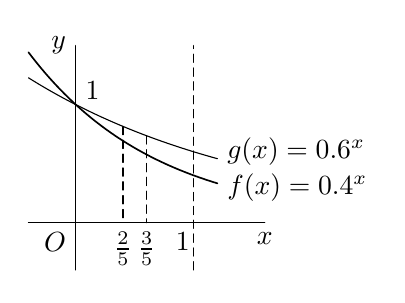
\begin{tikzpicture}[line cap=round,line join=round,scale=1.5]
      \draw[\myaxisarrow] (-0.4,0) -- (1.6,0) node[below] {$x$};
      \draw[\myaxisarrow] (0,-0.4) -- (0,1.5) node[left] {$y$};
      \draw[line width=0.6pt,smooth,samples=100] 
        plot[domain=-0.4:1.2](\x,{0.4^(\x)});
      \draw[line width=0.4pt,smooth,samples=100] 
        plot[domain=-0.4:1.2](\x,{0.6^(\x)});
      \draw[densely dashed] (1,-0.4)--(1,1.5) 
        (0.4,0.6^0.4)--(0.4,0) node[below] {$\frac25$}
        (0.6,0.6^0.6)--(0.6,0) node[below] {$\frac35$};
      \draw (0,0) node[anchor=north east] {$O$}
        (1,0) node[below,xshift=-4pt] {$1$} 
        (0,1) node[right,yshift=5pt] {$1$}
        (1.2,0.3) node[right] {$f(x)=0.4^x$} 
        (1.2,0.6) node[right] {$g(x)=0.6^x$};
    \end{tikzpicture}\end{center}}
    $g(x)= \Big(\frac35\Big)^x= 0.6^x$ 的图象知, 
    $\Big(\frac35\Big)^{\frac35}$ 与 $\Big(\frac25\Big)^{\frac25}$ 的值均介于 $\Big(\frac25\Big)^{\frac35}$ 和 $\Big(\frac35\Big)^{\frac25}$ 之间. 由 $\Big(\frac25\Big)^2< \Big(\frac35\Big)^3$ 知 $\Big(\frac25\Big)^{\frac25}<\Big(\frac35\Big)^{\frac35}$, 所以
    \[\Big(\frac25\Big)^{\frac35}< \Big(\frac25\Big)^{\frac25}< \Big(\frac35\Big)^{\frac35}< \Big(\frac35\Big)^{\frac25}.\]
    \mymarginpar{比较 $\Big(\frac35\Big)^{\frac35}$ 与 $\Big(\frac25\Big)^{\frac25}$ 的大小时, 无法利用 $y=x^x$ 或 $y=x\ln x$ 的单调性 (为什么\,?).}
  \endsolution
  
  \subsection{课后练习}
  
  \begin{exercise}
    若函数 $f(x)=(a^2 -3)^x$ 在 $\mathbb{R}$ 上单调递减,
    则实数 $a$ 的取值范围是\,?
  \end{exercise}

  \beginsolution
    $0<a^2-3<1$, 则 $a\in(-2,-\sqrt3)\cup(\sqrt3,2)$.
  \endsolution
  
  \begin{exercise}
    当 $a>0$ 且 $a\neq1$ 时, 函数 $f(x)=a^{x-2}+x+1$ 必过哪个定点\,?
  \end{exercise}

  \beginsolution
    由 $a^0=1$ 知 $f(2)=3$, 即 $f(x)$ 必过点 $(2,3)$.
  \endsolution
  
  \begin{exercise}
    若 $f(x)=5^{|x|}$, $g(x)=ax^2 -x$ ($a\in\mathbb{R}$),
    且 $f(g(1))=1$, 则 $a=$\,?
  \end{exercise}

  \beginsolution
    $f(g(1))=5^{|a-1|}=1$, 则 $a=1$.
  \endsolution
  
  \begin{exercise}
    计算: $0.027^{-\frac13}- \Bigl(-\frac17\Bigr)^{-2}
      + 256^{\frac34}- 3^{-1}+ (\sqrt3+1)^0$.
  \end{exercise}

  \beginsolution
    原式 $=\frac{10}3-49+64-\frac13+1=19$.
  \endsolution
  
  \begin{exercise}
    若直线 $y=2a$ 与函数 $y=|a^x -1|$ ($a>0$ 且 $a\neq1$) 
    的图象有两个公共点, 则实数 $a$ 的取值范围是\,?
  \end{exercise}

  \beginsolution
    分类讨论,并作 $f(x)$ 的图象知 $0<2a<1$, 即 $a\in\Big(0,\frac12\Big)$.
  \endsolution
  
  \begin{exercise}
    解方程: (1) $7\cdot 3^x=2(9^x-2)$;\quad (2) $\mathrm{e}^x+x=1$.
  \end{exercise}
  
  \beginsolution
    (1) $2\cdot(3^x)^2-7\cdot 3^x-4=0$, 则 $3^x=4$, $x=\log_3 4$.
    
    (2) $f(x)=\mathrm{e}^x+x$ 在 $\mathbb{R}$ 上 $\nearrow$, 
    \mymarginpar{方程可化为 $\mathrm{e}^x=1-x$, 由左边 $\nearrow$ 右边 $\searrow$ 知 $x=0$ 为唯一解.}
    而方程为 $f(x)=f(0)$, 故 $x=0$.
  \endsolution
  
%%%%%%%%%%%%%%%%%%%%%%%%%%%%%